% ------------------------------------------------------------------------
% file `main-bookexercise-7-solution-body.tex'
%
%     solution of type `bookexercise' with id `7'
%
% generated by the `exerciseanswer' environment of the
%   `xsim' package v0.21 (2022/02/12)
% from source `main' on 2026/10/26 on line 2278
% ------------------------------------------------------------------------
1. 选B。每一步所选的点，及选完该点后所有点的当前已知最短路径cur\_mind[]如下图所示（带下划线的数字表示该顶点的cur\_mind[]）。
\begin{center}
    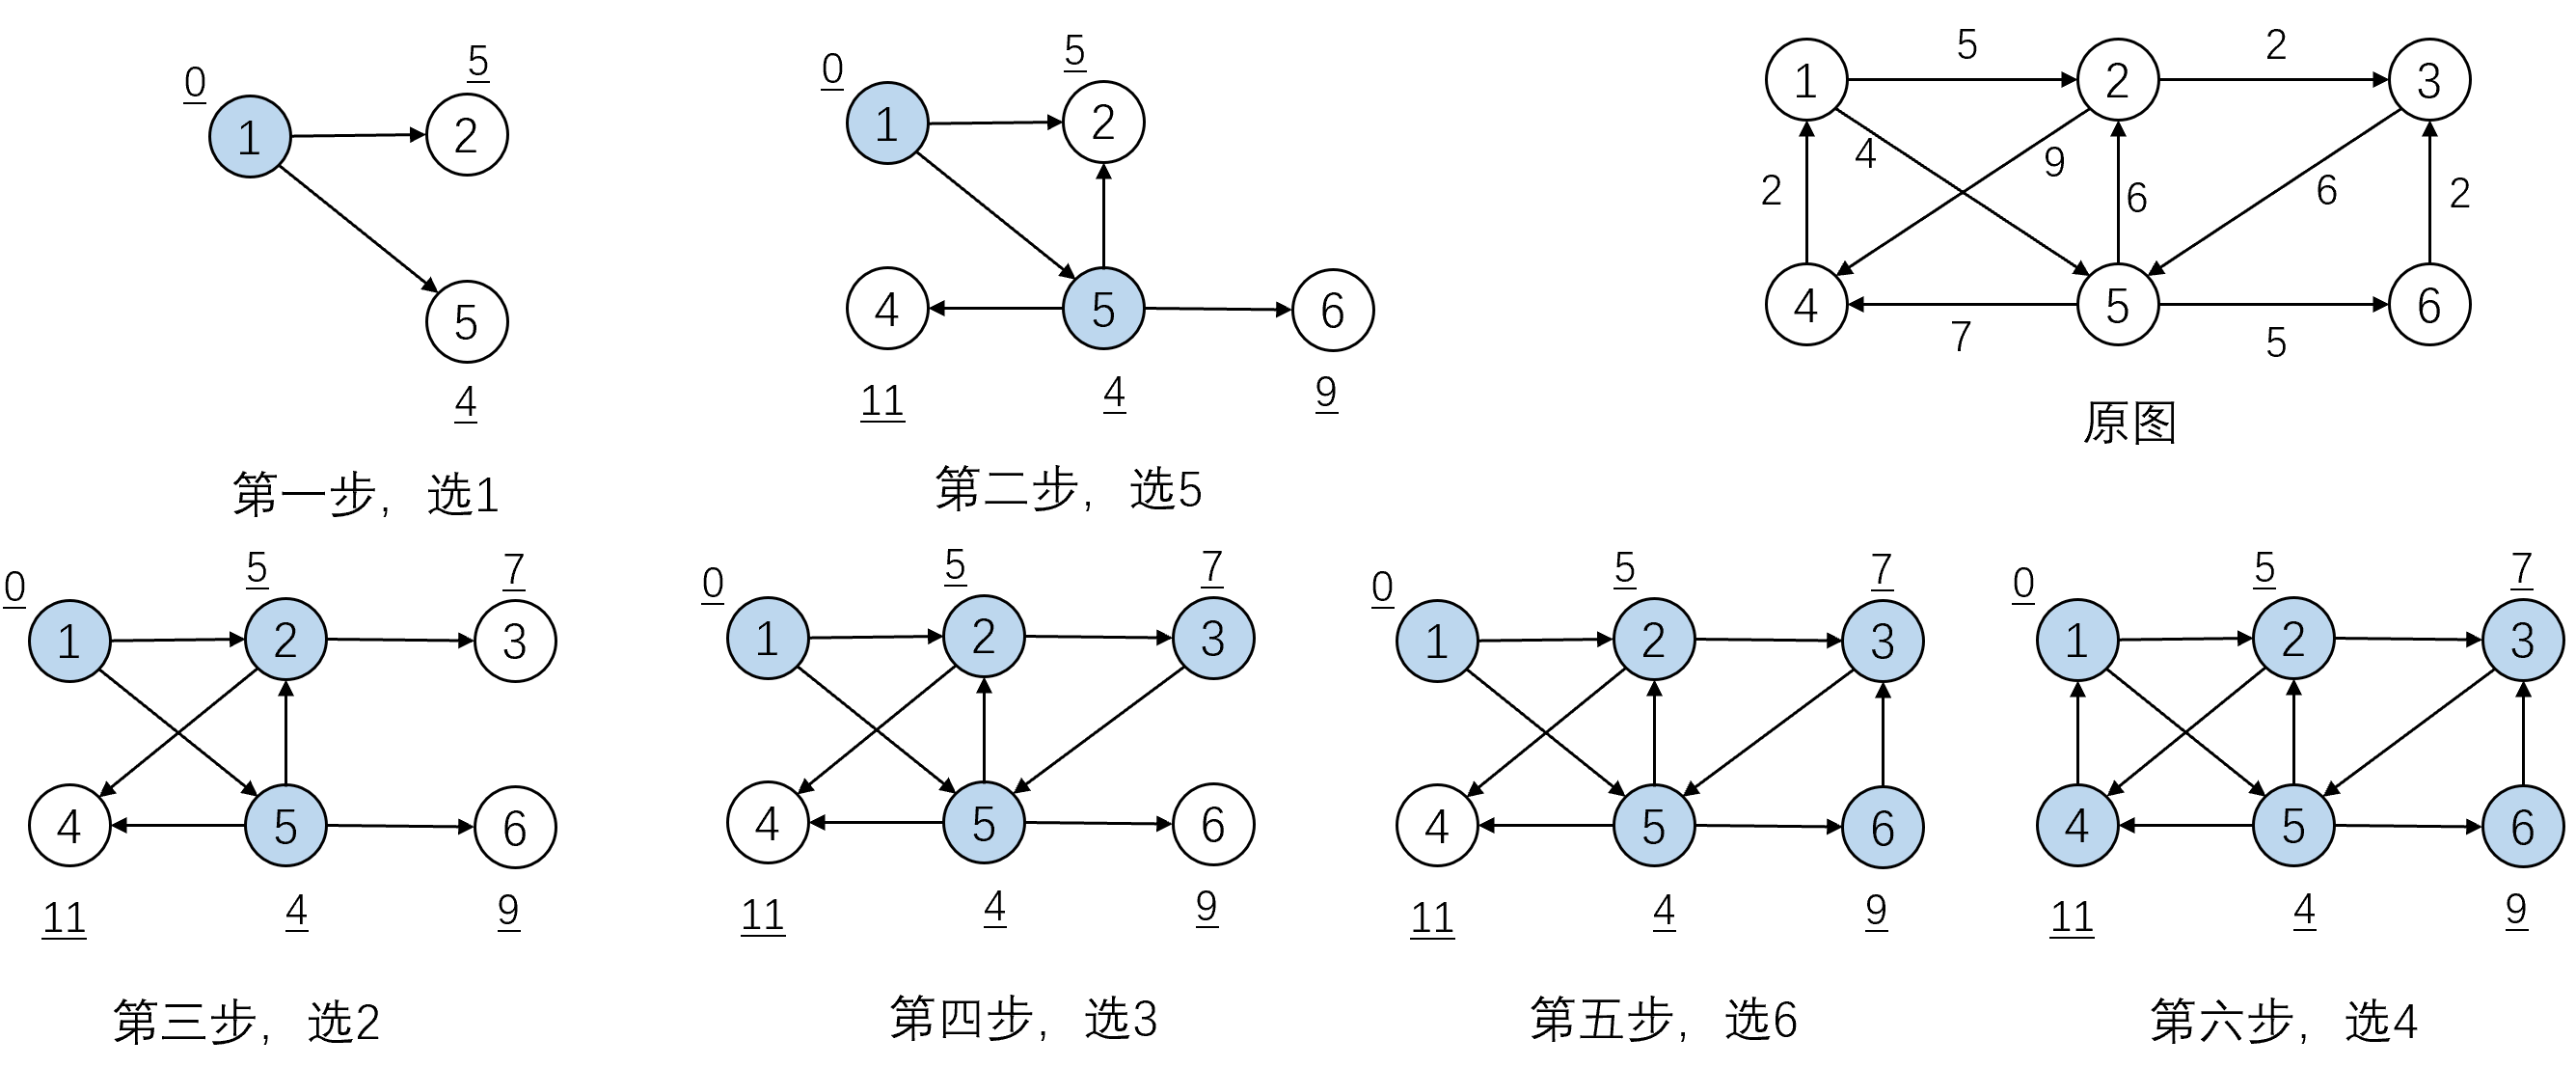
\includegraphics[width=1.02\textwidth]{assets/pics_and_ppts/ch5/习题09，16408最短路径的选点顺序答案图.png}
\end{center}
于是选点顺序是1,5,2,3,6,4，选B。\\

2. 选C。需要注意c到f是有一条边的，别看漏了就行。\\

3. 选C。求解前两个顶点（不包括源点）的最短路径过程如下所示。
\begin{center}
    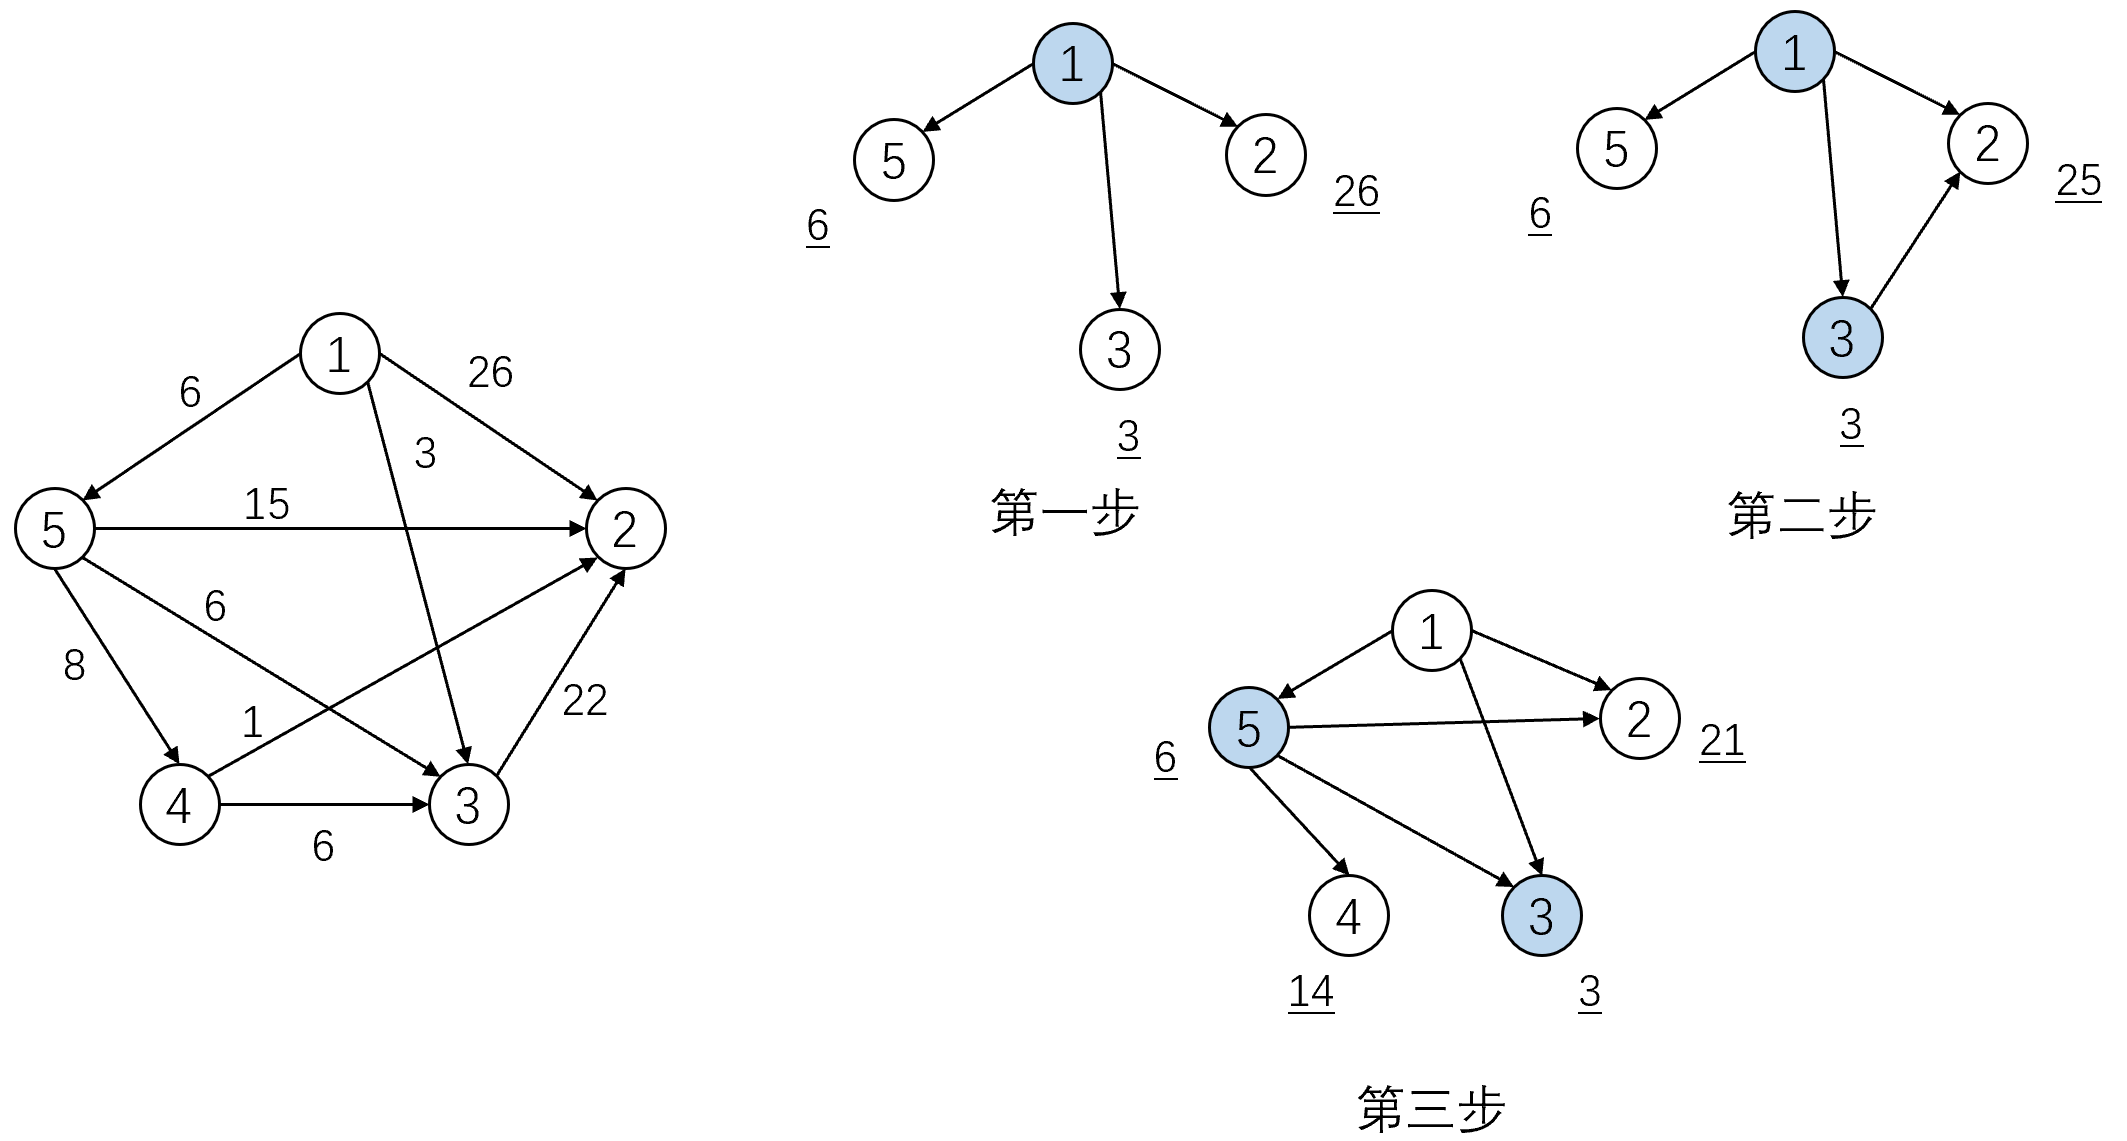
\includegraphics[width=0.95\textwidth]{assets/pics_and_ppts/ch5/习题11，21408迪杰斯特拉dist内容答案图.png}
\end{center}


